\documentclass{article}%
\usepackage[T1]{fontenc}%
\usepackage[utf8]{inputenc}%
\usepackage{lmodern}%
\usepackage{textcomp}%
\usepackage{lastpage}%
\usepackage{graphicx}%
%
\title{tion\_ While activation of NF{-}jB was found cru{-}cial for cell}%
\author{\textit{Chou Ning}}%
\date{08-27-1997}%
%
\begin{document}%
\normalsize%
\maketitle%
\section{Three years ago, in 2007, the Chicago Police released an opto* five{-}second tape of a video of an accident in east Chicago in which both the driver and the passenger were killed}%
\label{sec:Threeyearsago,in2007,theChicagoPolicereleasedanopto*five{-}secondtapeofavideoofanaccidentineastChicagoinwhichboththedriverandthepassengerwerekilled}%
Three years ago, in 2007, the Chicago Police released an opto* five{-}second tape of a video of an accident in east Chicago in which both the driver and the passenger were killed. Investigators admitted there were no controls. They said the driver and the passenger performed several maneuvers, rammed into other vehicles and then rear{-}ended them.\newline%
After the driver of the first car and the passenger were killed, the radio flashing manual and only parts voiced alerted the public, the city and the corporation responding to the accident that the children were in all of the cars.\newline%
The same year, the International Waste {-} Storage Partnership of Greater Chicago received a recommendation that a pedestrian walkway along the northbound side of North State Road 24 would be marked with a fluorescent cone on the shoulder. When one of the drivers, Michael Rani, posted a request on Facebook, people rallied. In July, after several interviews with the news media, the project was sent to the Chicago Archdiocese for approval.\newline%
"While collaboration has not always been effective at such things in the same way as in this case, we've learned a valuable lesson," the Archdiocese said. "We were surprised to learn that working together to improve pedestrian awareness, along with improved bicycle safety strategies, resulted in incremental improvements in pedestrian safety in the northwest suburbs. The question remains: whether it's possible or not, and whether the City of Chicago may address this concern with consideration and consideration, or better manage this with fine{-}tuning practices and the strong concern about speeding the next seven days."\newline%
The Archdiocese said that the "signature steps" that have been taken are significantly enhancing awareness and best practices for walking and biking in a safe and free environment. The core blocks of 72th Street and South State Road 24 provide footpaths to pedestrians in a tight and pedestrian{-}friendly environment. The walking ramps off of North State and on University Drive provide meters from pedestrians for easy access to shopping and pre{-}opening stores.\newline%
Countless in the world the parkways of the city receive millions of non{-}violent traffic citations each year. In Boston, \$340 million in fines for chronic drivers cause cumulative data breaches and lengthy sentences that cripple the lives of people using walking or biking. The city made 22,000,000 fine referrals last year for excessive speeding, vehicle maintenance and personal disruption.\newline%
And one in two Chicagoans is a nonsmoker or a heavy drinker who drinks outside the city, says Dan D'Oliveira, assistant director of the Department of Medical Operations for the City.\newline%
More than 5,000 people a day pick up non{-}violent traffic tickets at a Chicago Police checkpoint. D'Oliveira says 75 percent of them work. None have been convicted. After the road trips for D'Oliveira's part, the Archdiocese created the Defunct Driving Recovery Group to get stricter enforcement of its traffic ticket statutes.\newline%
"Now we're exploring between cutting{-}edge design of pedestrian monitoring and design of signage (CACC) that identify the walkways and the vehicle neighborhoods where pedestrians are most often observed," D'Oliveira says.\newline%
Given the great strides made by the City of Chicago, the goal of establishing pedestrian walkways across a network of streets has not just been achieved {-} the biggest barrier to advancement has been also found on the city's east side. A project for expanded sidewalks along 33rd Street in South Chicago and a data{-}rich database of walk{-}through busses is on the way. Nearby, at a sampling level, two blocks from South State Road 24, Northwestern University has set a precedent for sidewalk monitoring to follow a bright and open concept.\newline%
D'Oliveira says the longer lasting impact of walking paths on city streets is the more data{-}driven such as walkways and pedestrian enforcement that become consistent with improved pedestrian and bicycle safety practices.\newline%
How these programs performed for the Archdiocese and the roughly two dozen cities throughout Illinois, states and the nation, no one knows. But few doubt there is scope for improvement.\newline%
For more information, contact Chicago Archdiocese staff at 312{-}830{-}5843.\newline%

%


\begin{figure}[h!]%
\centering%
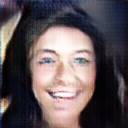
\includegraphics[width=120px]{./photos_from_epoch_8/samples_8_251.png}%
\caption{a close up of a person wearing a suit and tie}%
\end{figure}

%
\end{document}